\section{Speed Acquisition Channel}\label{sec:speed-acquisition-channel}

	\subsection{CKP Signal Conditioning}\label{ssec:ckp-signal-conditioning-circuit}

		As mentioned in Section \ref{ssec:speedMeasurement}, a CKP sensor has a analog signal with variable amplitude. For this project the only important parameter to extract from the sensor output signal in order to obtain the wheel speed is its frequency (angular velocity). The most practical way to obtain this data is to use a tachometer interface circuit, for this project the LM2907 from \textit{Texas Instruments} \cite{lm2907-datasheet} will be used. LM2907 is a \textit{frequency-to-voltage} converter with a ground-referenced tachometer input with $\pm$28V maximum voltage, making it versatile for many different sensor models.
		
		\subsubsection{LM2907 Basic Tachometer Circuit}\label{sssec:lm2907-basic-tachometer-circuit}
			The conditioning circuit for this project was based on the \textit{Tachometer with Adjustable Zero Speed Voltage Output} on Figure \ref{fig:lm2907-minimum-component-tachometer} suggested by LM2907 datasheet \cite{lm2907-datasheet}.

			\begin{figure}[htbp]
				\centering
				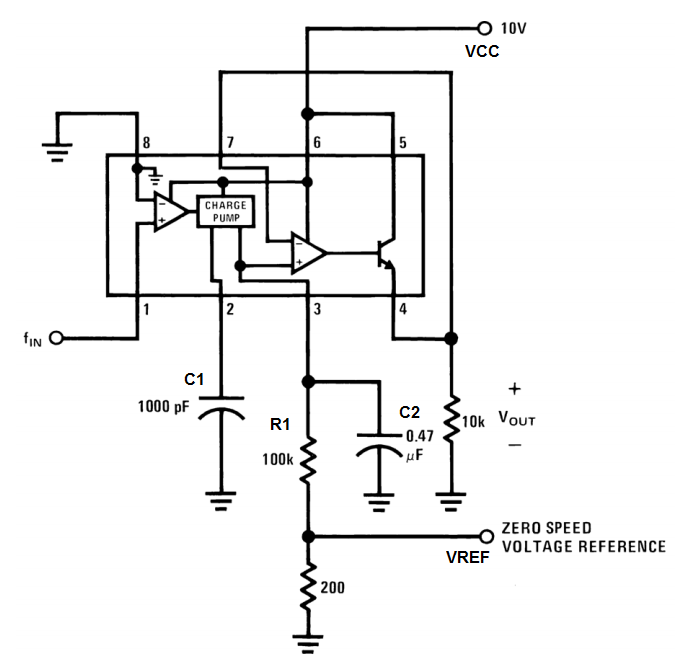
\includegraphics[width=.8\textwidth]{figuras/fig-lm2907-minimum-component-tachometer.png}
				\caption{Tachometer with Adjustable Zero Speed Voltage Output, adapted from \cite{lm2907-minimum-component-tachometer}}
				\label{fig:lm2907-minimum-component-tachometer}
			\end{figure}

			According to the datasheet (\cite{lm2907-datasheet}), in order to configure the gain of the frequency-to-voltage converter, C1, R1 and C2 must configured in respect to the following design requirements.

			\begin{itemize}
				\item\textbf{\textit{C1:}} This capacitor is charged and discharged every cycle by a 180$\mu$A typical current source. C1 must not be sized lower than 500-pF due to its role in internal compensation.\label{itm:lm2907-c1}
				\item\textbf{\textit{R1:}} Higher of R1 values increase the output voltage for a given frequency, but too large will degrade the output’s linearity. Because the current pulses are a fixed magnitude of 180 $\mu$A  typical, R1 must be big enough to produce the maximum desired output voltage at maximum input frequency. At maximum input frequency the pulse train duty cycle is 100$\%$, therefore the average current is 180 $\mu$A and R1 = Vo(max) / 180 $\mu$A.\label{itm:lm2907-r1}
				\item\textbf{\textit{C2:}} This capacitor filters the ripple produced by the current pulses sourced by the charge pump. Large values reduce the output voltage ripple but increase the output’s response time to changes in input frequency.\label{itm:lm2907-c2}
			\end{itemize}

			The output voltage ($V_{O}$) can be calculated using Equation \ref{eqn:lm2907-output-voltage}, $V_{CC}$ is the supply voltage and $f_{IN}$ the input frequency.

			\begin{equation}\label{eqn:lm2907-output-voltage}
				V_{O}=V_{REF} + \left( V_{CC} \cdot f_{IN} \cdot C1 \cdot R1 \right)
			\end{equation}

			As said in Item \ref{itm:lm2907-c2}, C2 controls the voltage ripple on the output($V_{RIPPLE}$), this ripple is given by Equation \ref{eqn:lm2907-ripple}. According to the datasheet, $I_{2}$ has a typical value of 180uA.

			\begin{equation}\label{eqn:lm2907-ripple}
				V_{RIPPLE}=\frac{V_{CC}}{2} \cdot \frac{C1}{C2} \cdot \left( 1 - \frac{V_{CC} \cdot f_{IN} \cdot C1}{I_{2}} \right)
			\end{equation}

			Finally, the last thing to consider is the maximum attainable input frequency, determined by $V_{CC}$, C1 and $I_{2}$ (180uA) in Equation \ref{eqn:lm2907-max-freq}.

			\begin{equation}\label{eqn:lm2907-max-freq}
				f_{MAX} = \frac{I_{2}}{C1 \cdot V_{CC}}
			\end{equation}

		\subsubsection{LM2907 Designed Circuit}\label{sssec:lm2907-designed-circuit}

			The first parameter to be calculated is the maximum frequency, functional requirement from Item \ref{itm:func-req-5} in Section \ref{sec:functionalRequirements} says the the system should be able to reach 200kph. Hence, to know the relation between frequency and speed on a wheel it's important to know the wheel's diameter.
			\par
			According to \cite{pneus-facil-todas-as-medidas-de-pneu}, the smallest commercial tyre size in terms of diameter in Brazil is the standard 165/70R13 which has a diameter (D) of 561.2mm and the one with the biggest diameter (D) is the standard 265/50R20 having 773mm. Using Equation \ref{eqn:diameter-to-length} to calculate the overall length of the wheel gives a aproximately length of 1.762m for the smaller tyre and a aproximately length of 2.428m for the bigger one.

			\begin{equation}\label{eqn:diameter-to-length}
				C = \pi \cdot D
			\end{equation}

			Considering this upper limit speed of 200kph, calculated values of tyre circumference length, we have maximum frequencies of aproximately 31.52Hz (for the smaller tyre standard) and 22.88Hz (for the bigger tyre standard). 
			\par
			According to \cite{lm2907-datasheet} the input common mode voltage is equal to $V_{CC}$ - 1.5V, and as $V_{CC}$ is equal to 5V (check Section \ref{sssec:5v-supply}) the maximum output voltage $V_{O}$ is equal to 3.5V. Considering a safer upper frequency limit of 60Hz (approximately double of the maximum calculated frequency of 31.52Hz) applied to Equation \ref{eqn:lm2907-output-voltage} with the $V_{CC}=5V$, the desired offset voltage $V_{REF}$ (1.225V, check Section \ref{sssec:1v2-reference}) and the maximum output voltage $V_{O}=3.5$ gives a time constant (R1*C1) of 0.0379. Using commercial resistor and capacitor values it is possible to achieve this time constant using C1=100nF and R1=374k$\Omega$, with this values $V_{O}$ can be described by Equation \ref{eqn:calculated-vo}.

			\begin{equation}\label{eqn:diameter-to-length}
				V_{O}=1.225V + 0.0374 \cdot f_{IN} V\/Hz
			\end{equation}

			For instance applying the upper frequency value of 31.52Hz calculated previously will give a $V_{O}=2.403V$.
			\par
			According to \ref{sec:mcu-hw}, the choosen microcontroller's ADC has a resolution of 10-bit. A analog reference of 5V with 10-bit resolution gives a voltage resolution of 4.88mV. Hence, the calculated voltage ripple of the frequency-to-voltage converter must be less than the ADC resolution. Using values o $V_{RIPPLE}$, C1, R1, $f_{IN}$ and $V_{CC}$ in Equation \ref{eqn:lm2907-ripple} gives a C2 value of aproximately 10$\mu$F.
			\par
			Figure \ref{fig:ckp-conditioning-circuit} shows the designed circuit for the speed acquisition channel.

			\begin{figure}[htbp]
				\centering
				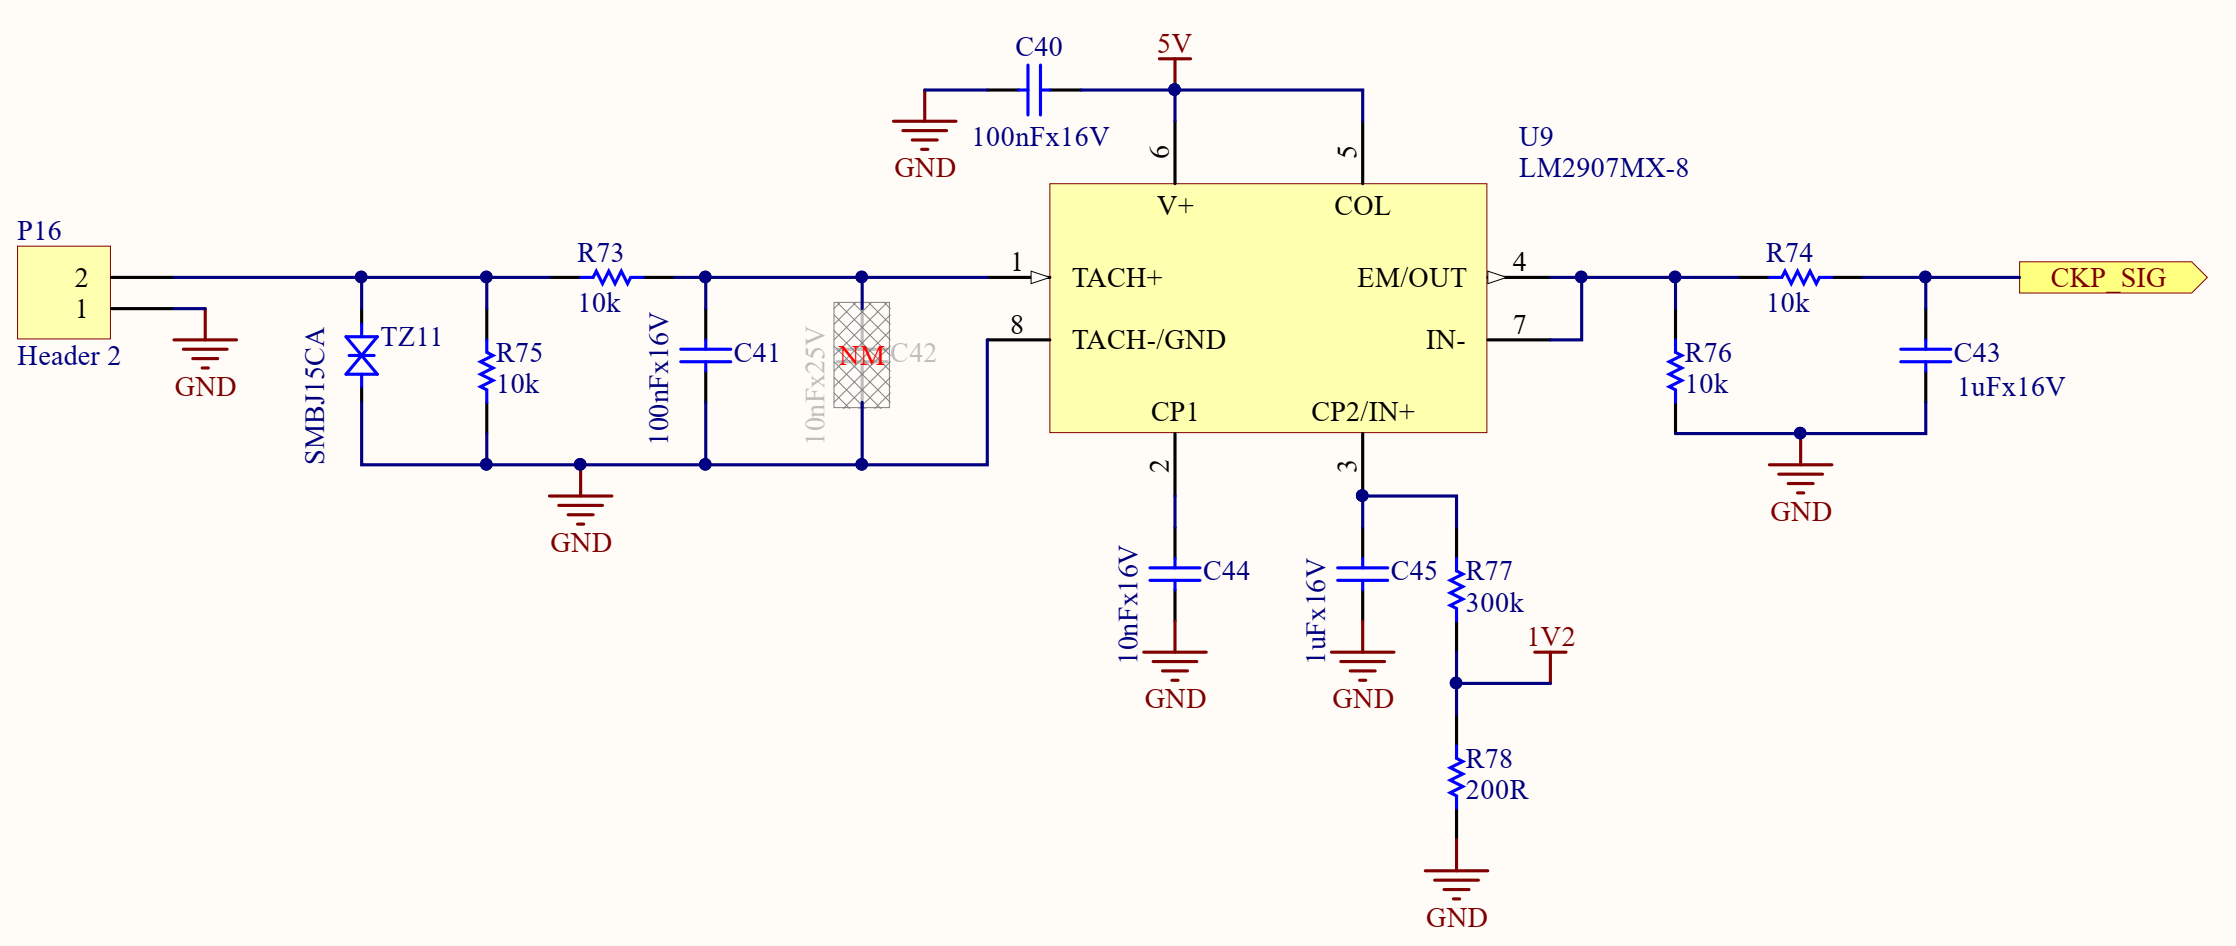
\includegraphics[width=.8\textwidth]{figuras/fig-ckp-conditioning-circuit.png}
				\caption{Speed Acquisition Channel Circuit}
				\label{fig:ckp-conditioning-circuit}
			\end{figure}

			In addition to the components from the circuit \textit{Tachometer with Adjustable Zero Speed Voltage Output} on Figure \ref{fig:lm2907-minimum-component-tachometer}, the following features have been added:

			\begin{itemize}
				\item\textit{\textbf{TVS Diode:}} In order to protect the the IC's input the SMBJ15CA TVS diode from \textit{Littelfuse} was added. This diode has a maximum clamping voltage of 26V, the maximum input voltage is $\pm$28V, thus the TVS will protect the input from overvoltages.\label{itm:ckp-circuit-tvs}
				\item\textit{\textbf{LPF at the input:}} As the maximum frequency was determined to be 31.52Hz, it is possible to filter all the upper frequencies in order to avoid any noise to enter the circuit. R73, C41 and C42 form a LPF with a cutoff frequency of aproximately 160Hz, this cutoff frequency was choosen because at 31.52Hz (maximum calculated input frequency), the attenuation is quite close to 0dB (-0.15dB) and shall not affect the input signal.\label{itm:ckp-circuit-lpf-input}
				\item\textit{\textbf{LPF at the output:}} R74 and C43 form a LPF to that is used to filter any external post-conversion noise, it has a aproximate frequency of 16Hz.\label{itm:ckp-circuit-lpf-output} 
				\item\textit{\textbf{R78:}} This resistor is recommended by \ref{lm2907-datasheet} in order to use the voltage reference functionality.\item{itm:reference-resistor}
			\end{itemize}


	\subsection{CKP Sensor Detection}\label{ssec:ckp-sensor-detection-circuit}

		The detection circuit consists basically of a filtered inverted digital input, a extra cable from the CKP ground will need to be wired in order to detect when the board sensor is connected.

		Figure \ref{fig:ckp-detection-circuit} shows the detection circuit for the CKP sensor.

			\begin{figure}[htbp]
				\centering
				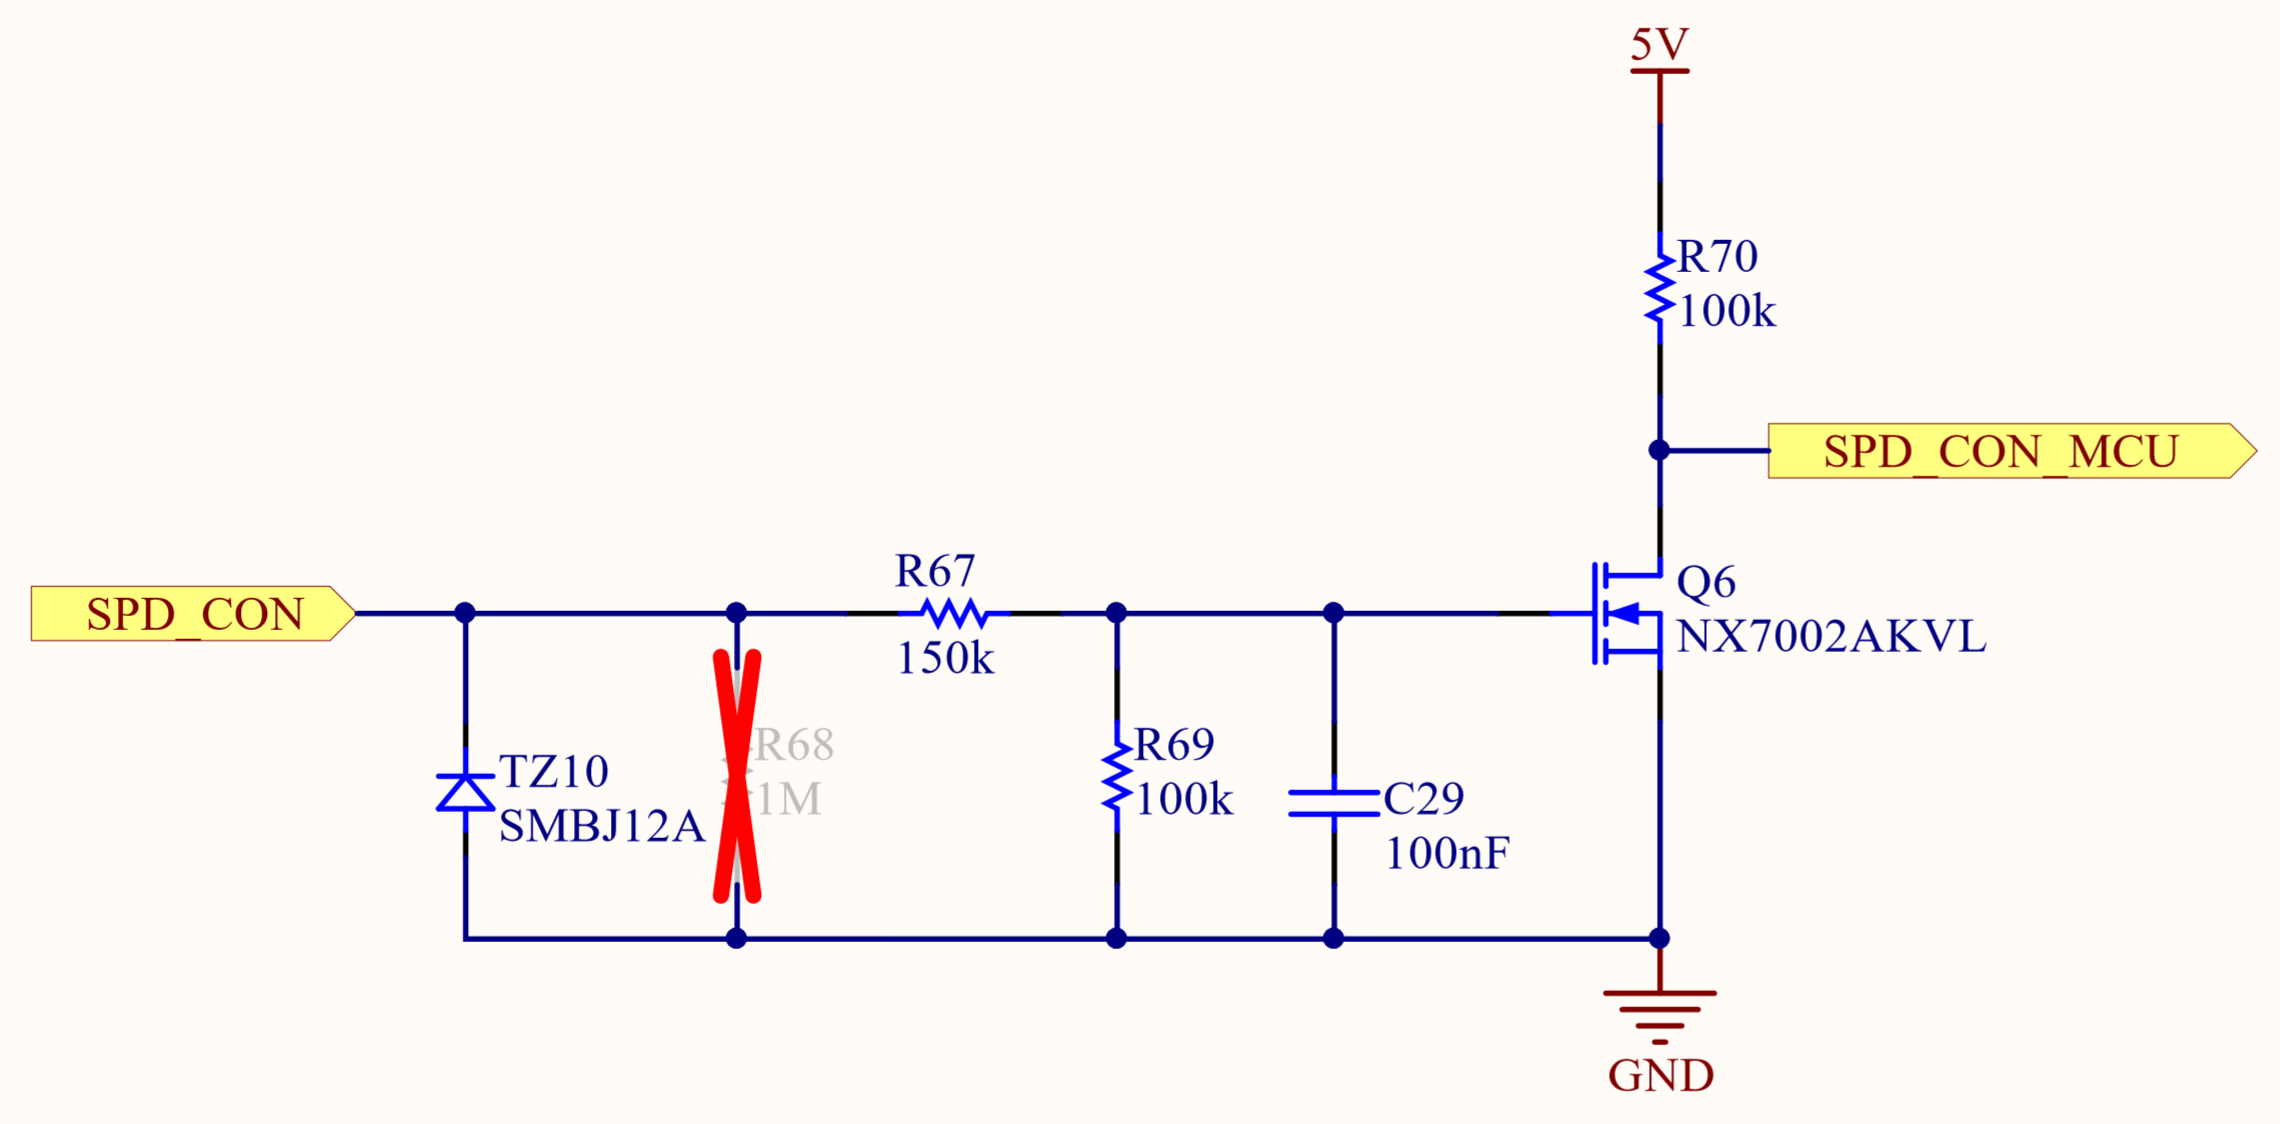
\includegraphics[width=.8\textwidth]{figuras/fig-ckp-detection-circuit}
				\caption{Speed Sensor Detection Channel Circuit}
				\label{fig:ckp-detection-circuit}
			\end{figure}

		The working principle of this circuit is this: when ground is connected to the input (sensor connected) the output goes to zero volts and the LED is turned ON, when high level voltage is connected to the input or it is on open load the output goes to high level and the LED turns off. D11 is a diode to guarantee that no transient voltage will flow from the input to the circuit. D13 is a additional protection clamping diode working alongside with the LPF formed by R81 and C46 to protect the Q17's gate.

	\subsection{1V2 Reference}\label{sssec:1v2-reference}

			The 1V2 reference from the circuit of Section \ref{ssec:ckp-signal-conditioning-circuit} is achieved using the LM4040CYM3-1.2 from \textit{Microchip} \cite{lm4040-datasheet}. This is a 1.225V precision voltage reference with a tolerance of $\pm 1.15\%$ and maximum operating output current of 10mA. The only external component needed is a bias resistor which can be calculated using \ref{eqn:rbis-adr510} \cite{lm4040-datasheet}.

			\begin{equation}\label{eqn:rbis-adr510}
				R_{BIAS} = \frac{V_{S} - V_{OUT}}{I_{L} - I_{Q}}
			\end{equation}

			The used $V_{S}$ \textit{Voltage Supply} will be the 5V obtained in the circuit from Figure \ref{fig:tl2575-05-circuit} in Section \ref{sssec:5v-supply}. According to the datasheet, the minimul operating voltage ($I_{Q}$ in this case) is 100uA. Moreover, $V_{OUT}$ is naturally 1.225V. The minimum bias current (load current $I_{L}$) is of 500nA (according to the \cite{lm2907-datasheet}). Hence, any value of resistance that guarantee that the current that flows through the regulator is less than 10mA is acceptable.
			\par
			Using a 1k$\omega$ resistor a current of 4mA can be achieved. Figure \ref{fig:1v2-circuit} shows the circuit for the 1V2 reference, the capacitors are just a bypass capacitors recommended by the datasheet.

			\begin{figure}[htbp]
				\centering
				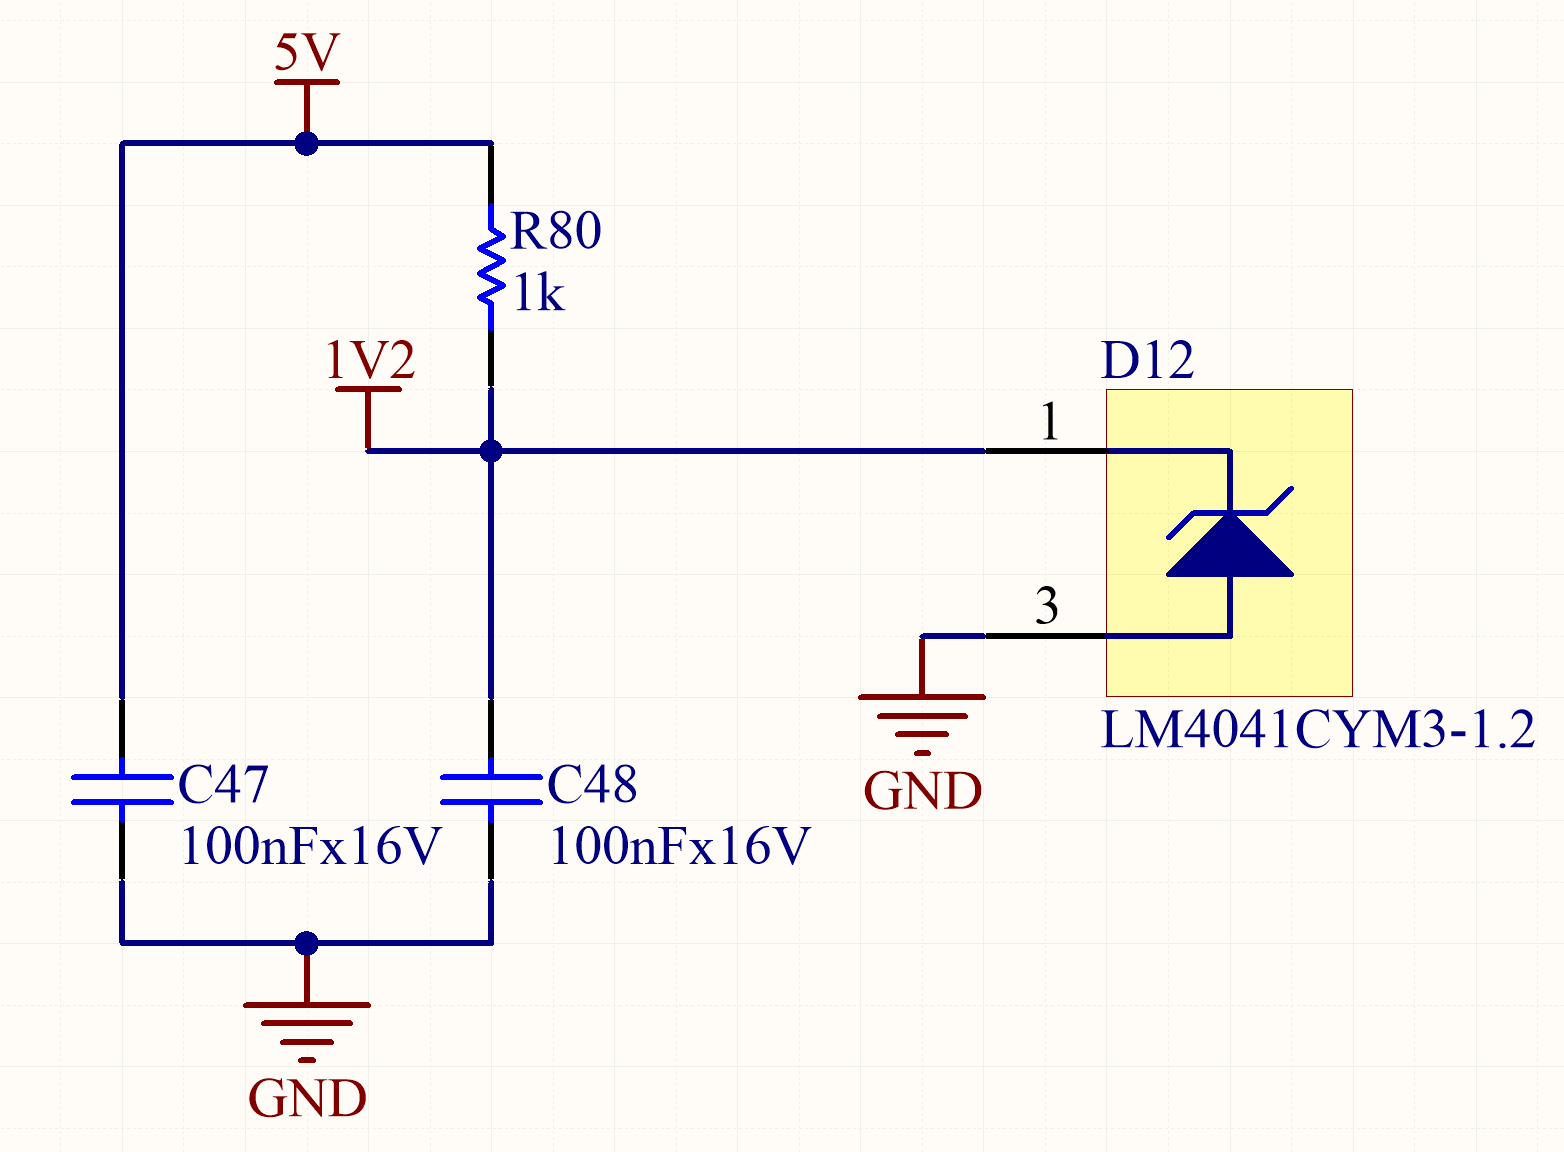
\includegraphics[width=.8\textwidth]{figuras/fig-1v2-circuit}
				\caption{1V2 voltage reference circuit}
				\label{fig:1v2-circuit}
			\end{figure}	 
